\chapter{Introdução}

	
A Computação Ubíqua, ou \textit{ubicomp}, vem sendo tema de diversas
pesquisas desde o início dos anos 90. Mark Weiser~\cite{weiser1, weiser2} diz que o computador do futuro deve ser
algo invisível, permitindo ao usuário focar mais na tarefa a ser desempenhada do que no uso da tecnologia para tanto.
A \textit{ubicomp} tem como objetivo concretizar esta invisibilidade tecnológica criando cenários onde o computador se integra a ambiente físicos juntamente com o apoio de softwares especializados de modo a constituir ambientes inteligentes. Tais ambientes, também chamados de \textit{smart spaces}, interagem com seus usuários e respectivos dispositivos, provendo serviços de modo proativo e transparente.

%  A Ubicomp
% tenta atribuir tal invisibilidade aos computadores criando uma realidade na qual
% o computador se integra a ambientes físicos constituindo os ambientes
% inteligentes que interagem com seus usuários e possuem uma ampla e transparente
% interação entre dispositivos e serviços disponíveis. A estes ambientes
% inteligentes é dado o nome de \textit{smart space}, cujo objetivo é auxiliar o
% usuário em suas tarefas utilizando os recursos
% disponíveis~\cite{fabriciobuzzeto,alegomes,weiser1, weiser2}.
	
A inteligência presente em um \textit{smart space} é fruto de aplicações que levam em consideração as informações de contexto do ambiente, isto é, informações sobre os usuários e dispositivos. Neste cenário, camadas de softwares denominadas de \textit{middlewares} são responsáveis por orquestrar a interação e troca de informações entre aplicações, usuários e dispositivos. Dentre os inúmeros dados de contexto que podem ser extraídos do \textit{smart space} destacam-se a localização e identidade do usuário, que são fundamentais para a implementação de serviços proativos e personalizados. Além disso, estes dados viabilizam a concepção de soluções de segurança em ambientes inteligentes~\cite{saocarlos}.


 % Portanto,
% informações como posição do usuário e sua respectiva identidade são de grande
% valia para tornar possível a interação entre o usuário e os recursos presentes.
% Um ambiente ubíquo capaz de obter tais informações, pode prover uma
% personalização automática de acordo com as preferências do usuário e até mesmo
% prover um ambiente mais seguro com controle de acesso físico e prevenção de
% fraudes \cite{saocarlos}.
	
% Informações como estas são um desafio a \textit{ubicomp} devido a alta
% dinamicidade do ambiente, 

A obtenção de informações acerca da localização e identificação dos usuários em \textit{smart space} torna-se um desafio tendo em vista a dinamicidade do ambiente, onde usuários entram e saem a todo momento, além de interagirem entre si e
com diversos dispositivos. Com a utilização de sensores é
possível obter dados sobre os usuários, que podem ser utilizados em
sistemas de rastreamento, localização e identificação. Estas tarefas, em
conjunto, podem fornecer informações de contexto com as posições e as
identidades de cada usuário no ambiente.
	
Neste trabalho foi desenvolvido um sistema de reconhecimento facial, rastreamento e
localização de usuários para um ambiente inteligente gerenciado pelo Middleware \textit{uOS}~\cite{fabriciobuzzeto}. O sistema, denominado TRUE (\textit{Tracking and Recognizing Users in the Environment}), utiliza o
sensor \textit{Kinect}~\cite{kinect_microsoft} como dispositivo de entrada. Este, por
sua vez, fornece imagens de cor e de profundidade ao sistema. O Middleware \textit{uOS} é voltado para a adaptabilidade de serviços em ambientes inteligentes. Conforme apresentado na Figura~\ref{fig:uos}, o \textit{uOS} atua como uma camada entre aplicações e \textit{drivers}, sendo que estes agregam os serviços providos pelos dispositivos no ambiente.

\begin{figure}[htb]
		\begin{center}
			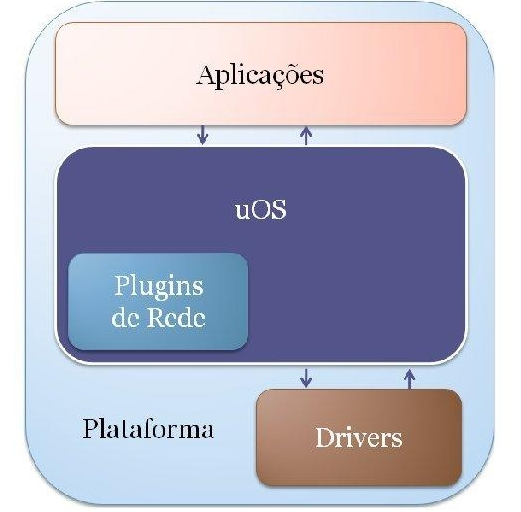
\includegraphics[scale=0.3]{figuras/1.Introducao/dsoa.jpg}
		\end{center}
		\caption{Middleware \textit{uOS}.}
		\label{fig:uos}
	\end{figure}

O restante desta monografia encontra-se organizado da seguinte maneira. No
Capítulo~\ref{cap:fundamentacao} são apresentados conceitos e técnicas sobre
rastreamento de entidades, localização e identificação das mesmas, além dos principais desafios da área. No
Capítulo~\ref{cap:trabalhos_correlatos} são analisados alguns projetos
relacionados a rastreamento, identificação e localização de pessoas em
ambientes inteligentes. O Sistema TRUE é apresentado no Capítulo~\ref{cap:true}, onde também são descritas as etapas de implementação e as soluções utilizadas para realizar rastreamento, localização e identificação de pessoas. Além disso, neste capítulo será detalhado a integração do Sistema TRUE com o Middleware \textit{uOS}. O Capítulo~\ref{cap:testes} descreve a condução de testes para validação do sistema bem como os resultados obtidos. Por fim, no Capítulo~\ref{cap:conclusao} são elencadas algumas considerações finais sobre este trabalho bem como sugestões de trabalhos futuros.


% O trabalho desenvolvido é apresentado no
% Capítulo~\ref{cap:true}, em que são descritos as diferentes etapas da
% implementação do Sistema TRUE e as soluções utilizadas para realizar
% rastreamento, localização e identificação de pessoas. Neste capítulo também é
% descrita em detalhes como a integração do sistema com o Middleware \textit{uOS}
% foi implementada. No Capítulo~\ref{cap:testes}, são apresentados os resultados
% dos testes realizados para validar a implementação do Sistema TRUE. Por fim, no
% Capítulo~\ref{cap:conclusao} são apresentados as considerações finais sobre este
% trabalho bem como sugestões de trabalhos futuros.


